\documentclass{article}

\usepackage{corl_2017}

\usepackage{natbib}
\usepackage[english]{babel}
\usepackage[utf8]{inputenc}
\usepackage{amsmath}
\usepackage{graphicx}
\usepackage[colorinlistoftodos]{todonotes}
\usepackage{booktabs}

\usepackage{tikz}
\usetikzlibrary{math,fpu,calc,fit,mindmap,backgrounds,positioning}

\usepackage{xspace}
\newcommand{\eg}{e.g.\xspace}
\newcommand{\etal}{et al.\xspace}
\newcommand{\ie}{i.e.\xspace}
\newcommand{\etc}{etc.\xspace}
\newcommand{\vs}{\textit{vs.}\xspace}

\graphicspath{{figs/}}

\title{PInSoRo: A Dataset for Deep-learning of Human-Robot Social Interactions}


\author{Séverin Lemaignan, Charlotte Edmunds, Tony Belpaeme}

\date{\today}

\begin{document}
\maketitle

\begin{abstract}

%% Original abstract -- kept for future reference
%Over the last decades, efforts around the world have sought to improve
%human-robot interactions, more recently with a focus on longer-term
%interactions. If worthy, these efforts are often incremental and many
%problems remain. In the light of the recent and rapid progress of machine
%learning, we propose here to shift the paradigm: instead of more and more
%complex symbolic cognitive modeling of the interactions between humans and
%robots, we argue that natural and sustainable human-robot interaction could
%instead be directly learned from actual human-human interactions. This paper
%outlines the main challenges ahead, and proposes a first concrete step
%toward the operationalisation of this novel paradigm: the creation of a
%large dataset of human-robot social interactions, suitable for machine
%learning.

Child-robot interactions are increasingly being explored in domains which
require longer-term application, such as healthcare and education. In order
for a robot to behave in an appropriate manner over longer timescales, its
behaviours should be aligned and meaningful to the interacting children.
Generating such sustained and engaging social behaviours is an on-going research
challenge, and we argue here that the recent progress of deep machine learning
opens new perspectives that the Human-Robot Interaction (HRI) community
should embrace.

As an initial step in that direction, we introduce a novel,
open dataset of children social interactions, designed with
machine learning applications in mind. Our data acquisition methodology relies on
a engaging and purposefully underspecified \emph{free play} interaction. By doing
so, we capture a rich set of behavioural patterns occurring in natural
social interactions. Learning to recognise, and possibly generate, such
behaviours is one of the future research direction that we foresee this dataset to effectively support.


\end{abstract}

\section{Machine Learning: the Next Horizon for Social Robots?}

While the family of recurrent neural networks (RNN) have repeatedly made the
headlines over the last few years with impressive results, notably in image
classification, image labelling and automatic translation, they have been so far 
largely ignored by  many other fields as they are perceived to require very
large datasets (hundreds of thousands to millions of observations) to actually
build up useful capabilities. Even though neural networks have demonstrated
compelling results in open-ended, under-specified tasks like image labelling, they
did not stand out as attractive approaches to problems involving high dimensions
with relatively small datasets available -- like human-robot social
interactions.

Besides, if one considers ``social interactions'' to also entail joint
behavioural dynamics, and therefore, some sort of temporal modeling, neural
networks look even less enticing as time is notably absent from most of the
tasks which neural networks have been successful at.

In 2015, the Google DeepMind team demonstrated how a convolutional
recurrent neural network could learn to play the game Break-Out (amongst
48 other Atari games) by only looking at the gaming console
screen~\cite{mnih2015human}. This result represents a major milestone: they show
that a relatively small sample size (about 500 games) is sufficient for an 
artificial agent to not only learn how to play (which requires an implicit model 
of time to adequately move the Break-Out paddle), but to also create gaming 
strategies that look like they would necessitate planning (the system first
breaks bricks on one side to eventually get the ball to break-out and reach out the area
above the remaining bricks, therefore ensuring rapid progress in the
game).

More recently, Ogata's team~\cite{yang2017repeatable} has demonstrated how an
adequately configured RNN is able to learn a complex robotic task (folding soft
objects like towels using a dual-arm mobile manipulator) from only \emph{35}
demonstrations of $\approx$ 70 seconds-long teleoperated
sequences. The network inputs are the raw video stream from the head camera and the
12 DoF of the two arms. Successfully folding towels entails an explicit sequencing of
actions (therefore implicit temporal modeling): the fact that such a complex
process can be successfully learned from a small training dataset should lead
us to reconsider the range of domains to which RNNs would be applicable.

Indeed, as we have previously argued~\cite{lemaignan2016towards}, we believe
that the complexity of mechanisms that such neural networks have been able to
uncover and model should invite our community to question its applicability to
human-robot interactions in general, and sustained, natural child-robot
interactions in particular. The current lack of appropriate HRI
datasets suitable for neural networks training is however an obstacle: we
introduce in this article the PInSoRo dataset, a large dataset of child-child
natural interactions suitable for machine learning.

\subsection*{Machine Learning and Social Behaviours}

The use of interaction datasets to teach robots how to socially behave has been
previously explored, and can be considered as the extension of the traditional
learning from demonstration (LfD) paradigms to social interactions (for
instance~\cite{nehaniv2007imitation,mohammad2015interaction}). Existing
research focuses however on low-level recognition or generation of short,
self-standing behaviours, including social gestures~\cite{nagai2005learning}
and gazing behaviours~\cite{calinon2006teaching}.

Based on a human-human interaction dataset, Liu \etal~\cite{liu2014how} have
investigated machine learning approaches to learn longer interaction sequences.
Using unsupervised learning, they train a robot to act as a shop-keeper,
generating both speech and socially acceptable motions. Their approach remains
task-specific, and while they report only limited success, they emphasise the
``life-likeness'' of the generated behaviours.
%They rely on unsupervised learning, with a
%training stage consisting in clustering behavioural states (a state consist in
%\emph{behavioural elements} (joint states of the two interacting agents,
%associated to the current speech elements, as well as the current joint
%\emph{spatial formation}), followed by the

These examples show the burgeoning interest of our community for the automatic
learning of social interactions, but also highlight the lack of structure of
these research efforts, as further illustrated by the lack of large, open
datasets of social interactions, suitable for machine-learning applications.

One interesting dataset is the \emph{Multimodal Dyadic Behavior
Dataset} (\emph{MMDB},~\cite{rehg2013decoding}). It comprises of 160 sessions of
3 to 5 minute child-adult interactions. During these interactions, the
experimenter plays with toddlers (1.5 to 2.5 years old) in semi-structured ways.
The dataset includes video streams of the faces and the room, audio, physiological data
(electrodermal activity) as well as manual annotations of certain behaviours
(like gaze to the examiner, laughter, pointing). The lack of calibration and camera positioning
information in the dataset limits the possibilities of automatically extracting and
labelling key interaction features (like facial expressions or joint gaze). Besides,
this dataset focuses on very young children with in adult-driven interactions,
and as such does not include any episodes of naturally-occurring social
interactions between peers.

\todo[inline]{look at other child-child datasets!}
\todo[inline]{mention research on deep-learning to diagnose autism}

\section{The Plymouth Interacting Social Robots Dataset (PInSoRo)}

\todo[inline]{the dataset is not specific to robotics...PinSoRo is maybe not the
    best name?}

The Plymouth Interacting Social Robots (PInSoRo) Dataset comprises of natural
social interactions arising between children, and recorded with machine learning
applications in mind.

As detailed in section~\ref{availability}, this dataset is open and made freely
available to any interested researcher. It is intended to be used to train
machine-learning algorithms (typically, deep recurrent networks) to both
recognise and generate complex cognitive and social dynamics occurring in the
wild during social interactions.

\subsection{The Freeplay Sandbox}

\begin{figure}
    \centering
    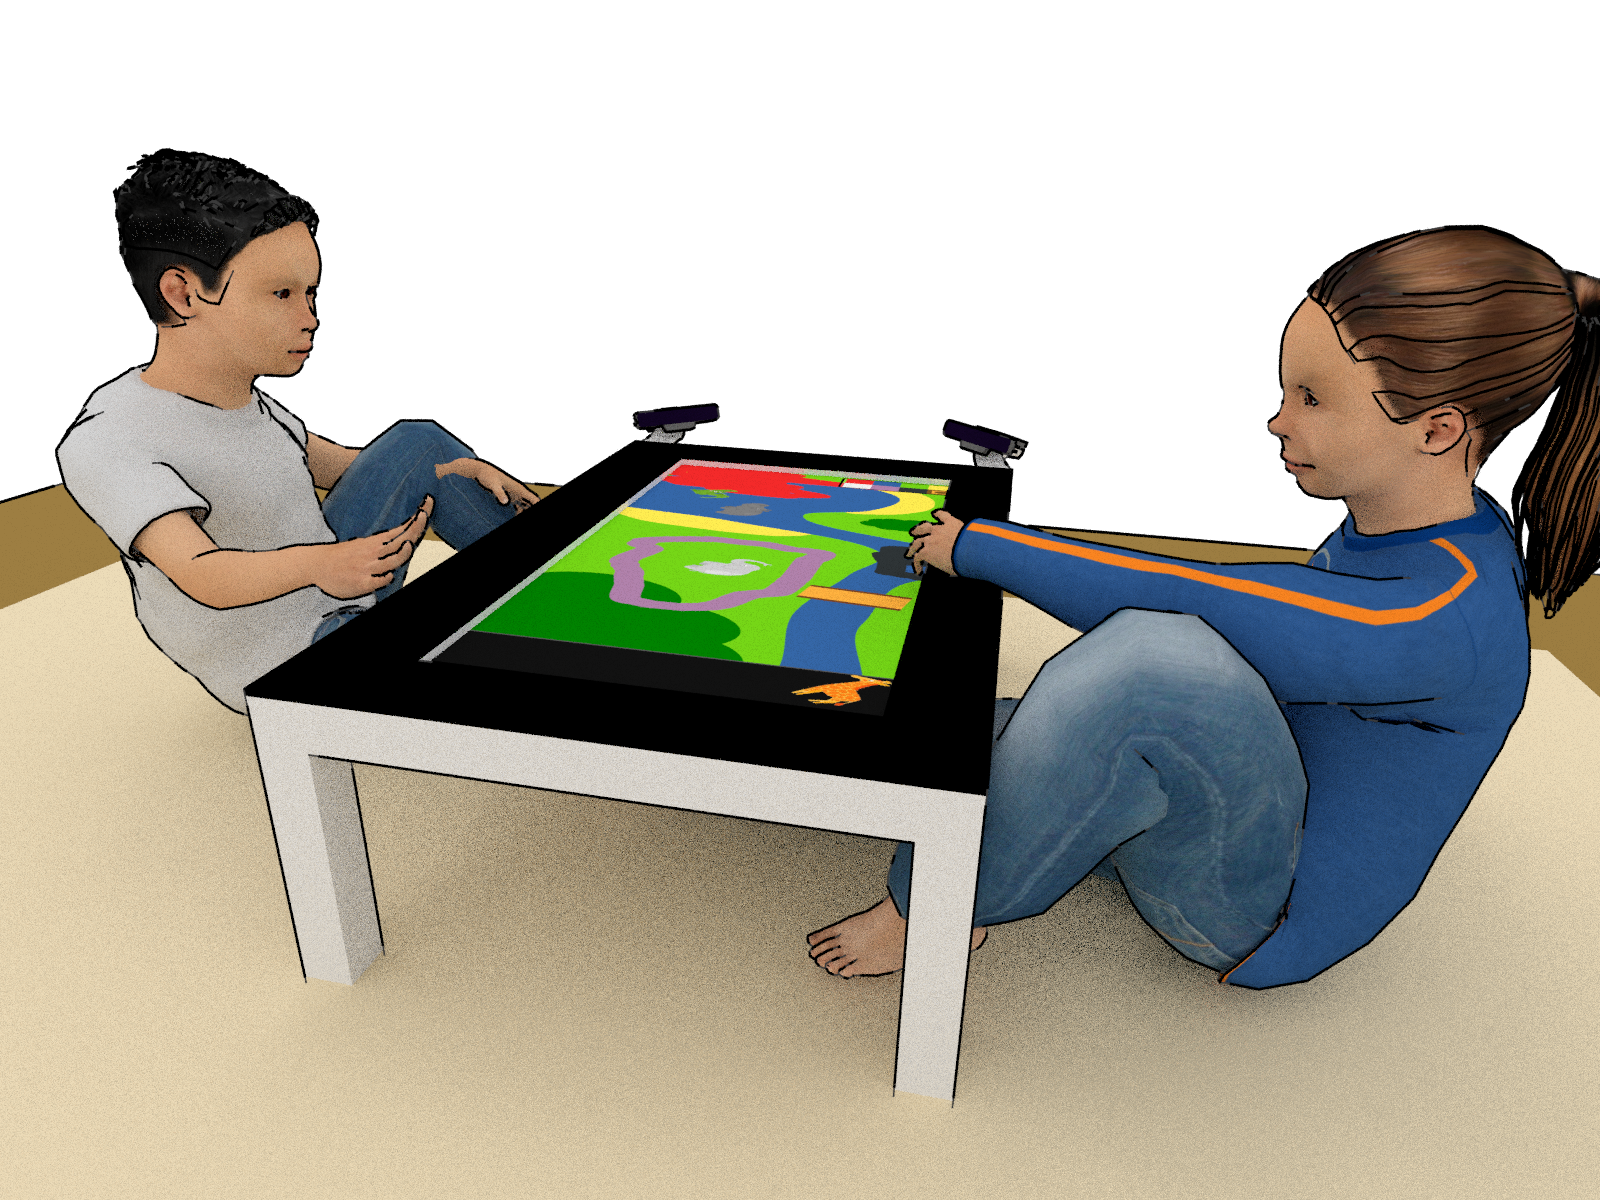
\includegraphics[width=0.55\linewidth]{setup-child-child.png}
    \hspace{1em}
    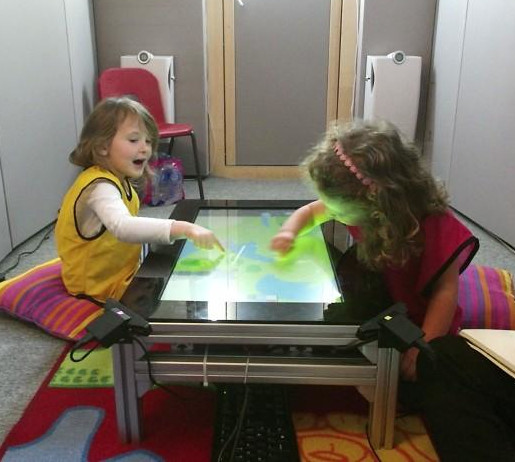
\includegraphics[width=0.4\linewidth]{child-child-env}
    \caption{The free play social interactions sandbox: two children interact in
    a free-play situation, by drawing and manipulating items on a touchscreen.}
    \label{fig|freeplay}
\end{figure}

The acquisition of such a dataset requires first the definition of a suitable
task for the participants to perform while they are recorded. The nature of
this task influences in fundamental ways the kind of interactions that might be
observed, and thus, learned. Because they usually target very specific social
or cognitive skills in a tightly controlled manner, traditional socio-cognitive tasks are
usually simple, constrained tasks that do not reflect the complexity and dynamics of
real-world interactions. On the contrary, this dataset aims at capturing a rich set
of naturally-occurring social interactions. As such, a suitable task has to be:

\begin{itemize}
    \item elicit a large range of interaction situations;
    \item foster rich multi-modal interaction: simultaneous speech, gesture, and gaze
        behaviours are to be observed;
    \item fundamentally social, \ie the task would make little sense for an
        agent alone;
    \item foster non-trivial social dynamics, such as implicit turn-taking.
\end{itemize}

We present a new experimental task based on \emph{free play} interactions. Pairs
of children (4-7 years old) are invited to freely draw and interact with items
displayed on an interactive table, telling and acting stories with no explicit
goal set in advance (Fig.~\ref{fig|freeplay}). The task is designed so that
children can engage in open-ended and non-directive play situations, yet
sufficiently well defined to be controlled, suitable for detailled recording,
and easily reproducible.

\begin{figure}[ht!]
    \centering
    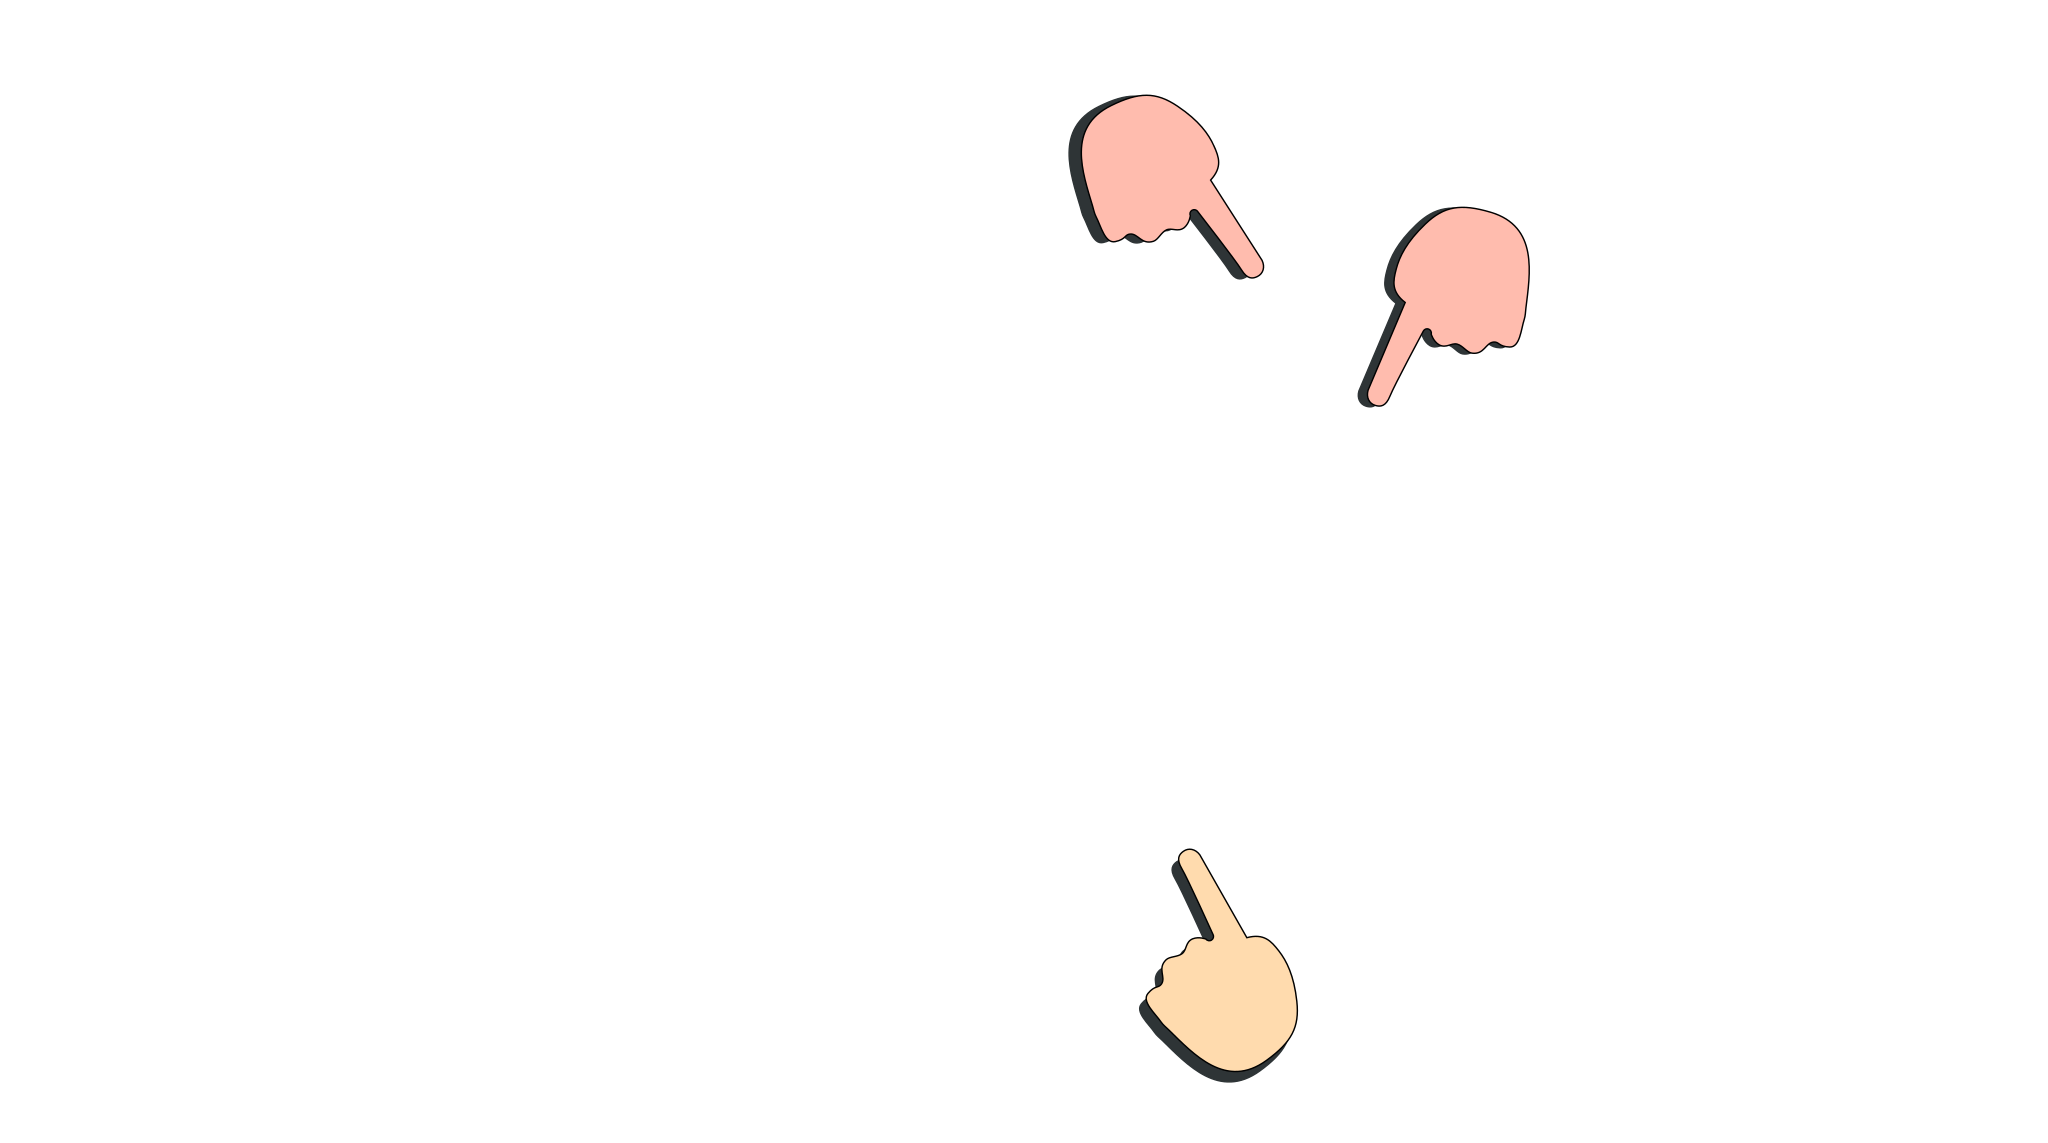
\includegraphics[width=0.8\linewidth]{sandbox}
    \caption{Example of a possible game situation. Items (animals,
    characters...) can be dragged over the whole play area, while the background
    picture can be painted over by picking a colour.}

    \label{fig|sandbox}
\end{figure}

The \emph{freeplay sandbox} follows the sandtray
paradigm~\cite{baxter2012touchscreen}: a large touchscreen (60cm $\times$ 33cm,
with multitouch support) is used as an interactive surface (\emph{sandtray}). The two children play together
by freely moving interactive items (Fig.~\ref{fig|sandbox}) on the surface. A background image
depicts a generic empty environment, with different symbolic colours (water,
grass, beach, bushes...). By drawing on top of the background picture, the
children can also alter this environment to their liking. The players do not have any particular task to
complete, they are simply invited to freely play for as long as they wish.

In order to constraint the dataset to a tractable domain, the task is limited to
a dyadic \emph{face-to-face} interaction.  The resulting interaction space is
nevertheless high-dimensional, with two main axis: the game-related actions
(drawing, manipulating items, telling stories) and the social interactions
(monitoring the other's actions, discussing and agreeing on joint actions,
helping behaviours, etc.).

%
%\paragraph{Socio-cognitive framing of the task}
%
%
%focus on abstract socio-cognitive facets (robot
%perception and manipulation are simplified); well suited for qualitative and
%quantitative analysis using metrics like Słowinski’s Individual Motor Signature
%(for behavioural alignment), Anderson's~\cite{anderson2004social} coding of children’s free-play
%interactions, with-me-ness (for assessment of co-engagment).
%
%carefully framed: as far as possible, they necessitate only the cognitive
%capabilities that they evidence (e.g. if they evidence a purely socio-linguistic
%mechanism, they will not mandate complex action capabilities – they may benefit
%from it, though),
%
%This point is especially important as it allows an incremental path: a robot
%should be able to tackle one or several of these task independently of the
%others, and a research team may progressively extend their cognitive models to
%incorporate more and more of the cognitive capabilities required by the robot to
%address all of the tasks.



\subsection{Dataset structure}

The dataset consists in a collection of records. Each record correspond to one
play interaction between two children. To date (June 2017) 25 records have been acquired (\ie 50 children). At the end of the acquisition campaign
(July 2017), the dataset is planned to include 50 records. As
mentioned above, the duration of each play episode varies ($M=20m51s,
SD=10m40s$), but it is capped to a maximum of 40 minutes.

Data is collected using the ROS middleware\footnote{\url{http://ros.org}} and
recorded as \emph{bag} files. Every dataframe is timestamped.
Table~\ref{table|datastreams} lists all the recorded datastreams.

\begin{table}[]
\centering
\caption{List of datastreams stored in each record}
\label{table|datastreams}
\begin{tabular}{@{}lll@{}}
\toprule
\bf Domain  & \bf Type                              & \bf Details                          \\ \midrule
child 1     & audio                                 & 16kHz, mono, semi-directional        \\
            & face (RGB)                            & qHD (960$\times$540), 30Hz           \\
            & face (depth)                          & VGA (640$\times$480), 30Hz           \\
            & facial features                       & 68 3D points (point cloud)           \\ \midrule
child 2     & audio                                 & 16kHz, mono, semi-directional        \\
            & face (RGB)                            & qHD (960$\times$540), 30Hz           \\
            & face (depth)                          & VGA (640$\times$480), 30Hz           \\
            & facial features                       & 68 3D points (point cloud)           \\ \midrule
environment & RGB                                   & qHD (960$\times$540), 29.7Hz         \\ \midrule
touchscreen & background drawing (RGB)              & 4Hz                                  \\
            & touches                               & 6 points multi-touch                 \\
            & items position and orientation        & ($x,y,\theta$)                       \\ \midrule
others      & \multicolumn{2}{l}{annotations of social behaviours and remarkable events}   \\
            & \multicolumn{2}{l}{static transforms between touchscreen and facial cameras} \\
            & \multicolumn{2}{l}{cameras calibration informations}                         \\ \bottomrule
\end{tabular}
\end{table}

As the data is recorded using ROS's bag files, it can be replayed in the exact
same conditions as it was during the recording. All the video streams use
calibrated cameras. Only the raw RGB and depth video streams are recorded. 

\subsection{Hardware and Software}

\paragraph{Hardware}
The sandtray is made of a 27" Samsung All-In-One computer running Ubuntu Linux
and equipped with a fast 1TB SSD hard-drive. The computer is held horizontal in
a custom aluminium frame standing 26cm above the ground
(Fig.~\ref{fig|freeplay}, right). All the cameras are plugged directly over
USB-3 to the computer. The computer performs all the data acquisition using ROS
Kinetic.

The children faces are recorded from two Intel RealSense SR300 RGB-D cameras
(short range, 0.2m to 1.2m, indoor RGB-D cameras), placed at the corners of the
the sandtray (Figs.~\ref{fig|rviz} and~\ref{fig|setup}), and tilted to face the
children. The cameras are rigidly mounted on custom 3D-printed brackets, and
their 6D pose with respect to the sandtray screen is precisely known and
recorded (this enables in particular accurate estimation of the children's head
pose).

Audio is recorded from the same SR300 cameras (one audio stream is recorded for
each child, from the camera facing her/him).

Finally, a third RGB camera (the RGB stream of a Microsoft Kinect One) records
the whole interaction setting. These video stream is intended to support human
coders while annontating the interaction, and is not precisely calibrated.

\begin{figure}[ht!]
    \centering
    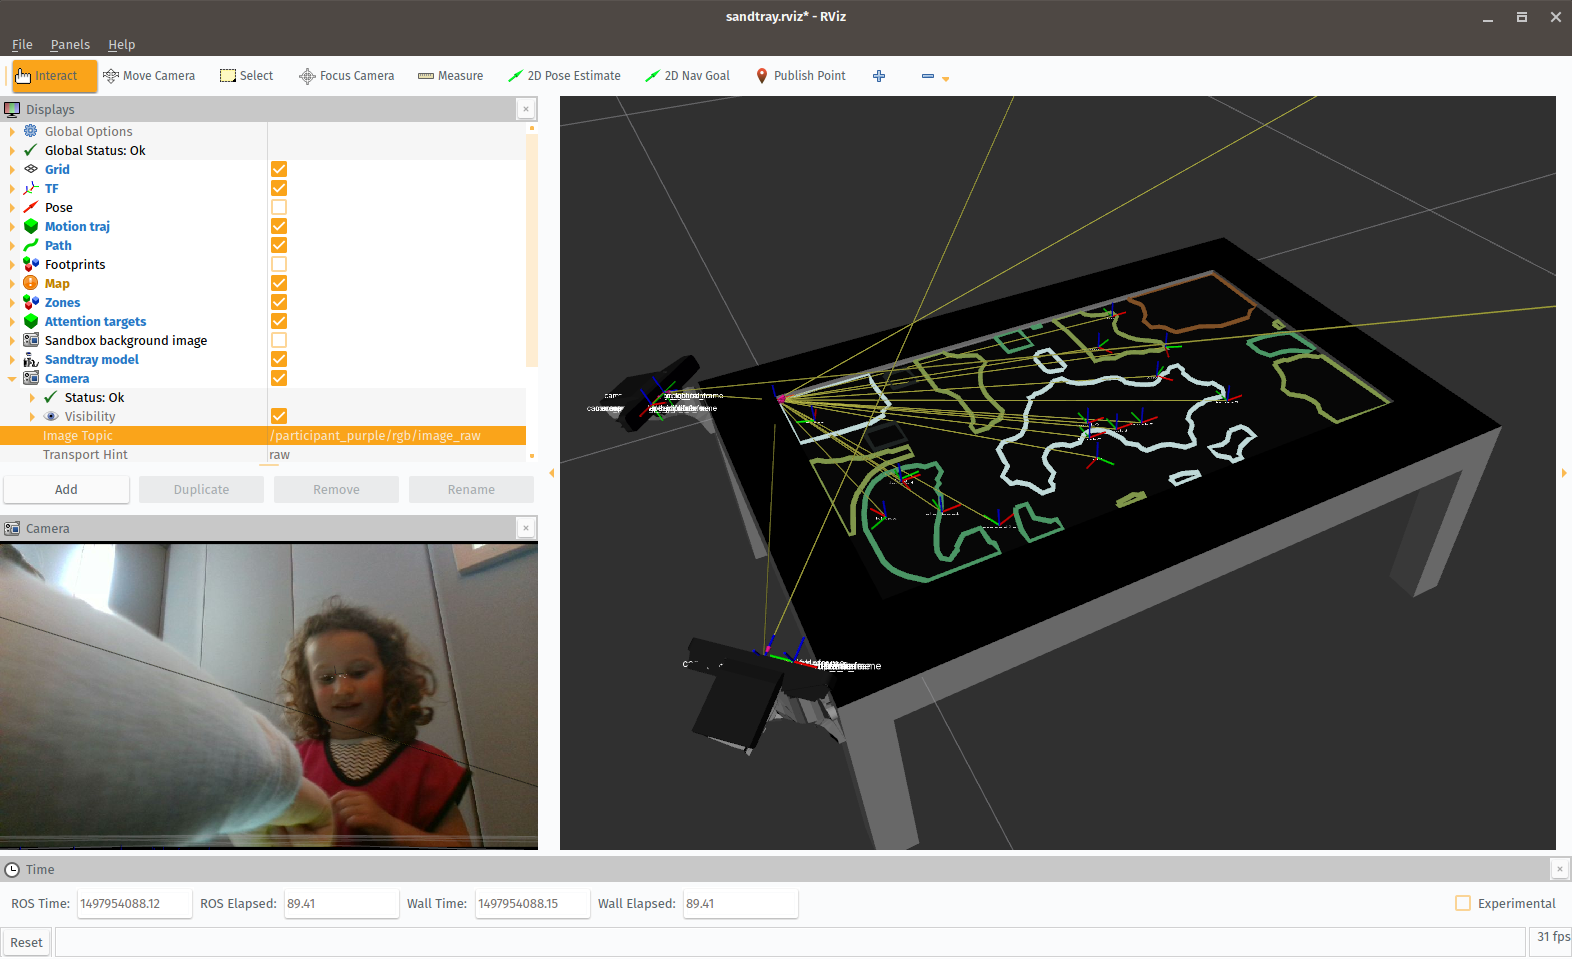
\includegraphics[width=0.5\linewidth]{rviz-sandtray}
    \hspace{0.2em}
    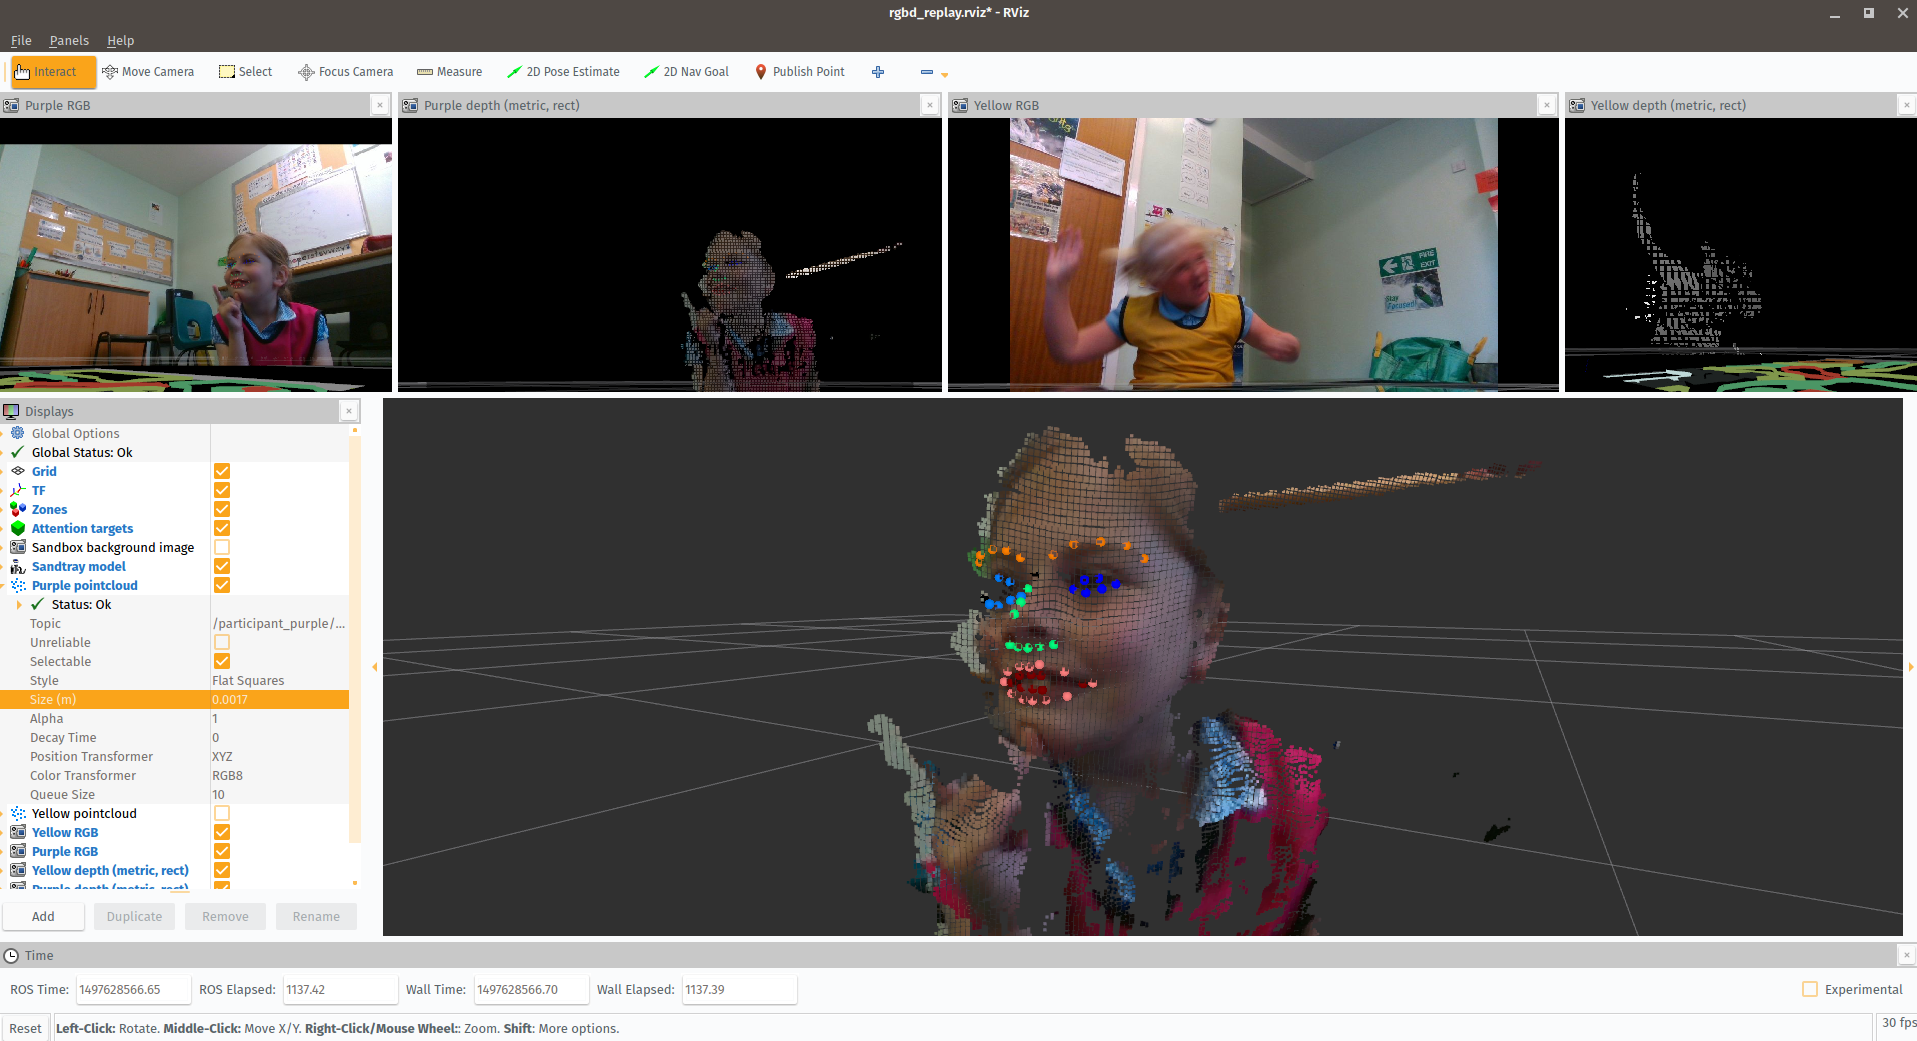
\includegraphics[width=0.48\linewidth]{3d-point-cloud-facial-features}
    \caption{The freeplay sandbox, visualised at runtime with ROS RViz. The
    current background drawing is published on a regular image
    topic and computer vision is used to segment it into zones (visible in
    the central panel, right picture). The poses of the interactive items
    are published, as well as an estimate of the children's head pose.
    The left picture shows a reconstructed 3D point cloud of one child face,
    along with the detected 68 facial features.}
    \label{fig|rviz}
\end{figure}

\paragraph{Software}
The sandbox is implemented with two frameworks: the Qt's \emph{QtQuick} framework
for the graphical interface of the game, and the \emph{Robot Operating System}
(ROS) for the modular implementation of the data processing and data acquisition
pipelines. A dedicated bridge between QtQuick and ROS has been specifically
developped to enable the game interface to export the positions of every
iteractive items as they move, the background image whenever it is painted over,
and the children's touches. The game interface is open-source and available online:
\url{https://github.com/severin-lemaignan/freeplay-sandbox-qt}.

By relying on ROS for the data acquisition, real-time monitoring of the
interaction is also possible (Fig.~\ref{fig|rviz}).
The ROS data acquisition pipeline is open-source as well, and available from
\url{https://github.com/severin-lemaignan/freeplay-sandbox-ros}.

Finally, we have developped a web-based \emph{supervisor} that permits the
experimenter to remotely start/stop the ROS nodes and the game GUI, as well as to
record annotations during the experiment. The supervisor ensures that the exact
same recording procedure (detailled in the next section) is followed for every
participants. The supervisor is available online as well:
\url{https://github.com/severin-lemaignan/freeplay-sandbox-supervisor}.

\subsection{Dataset Acquisition}

\begin{figure}[htbp]
    \centering
    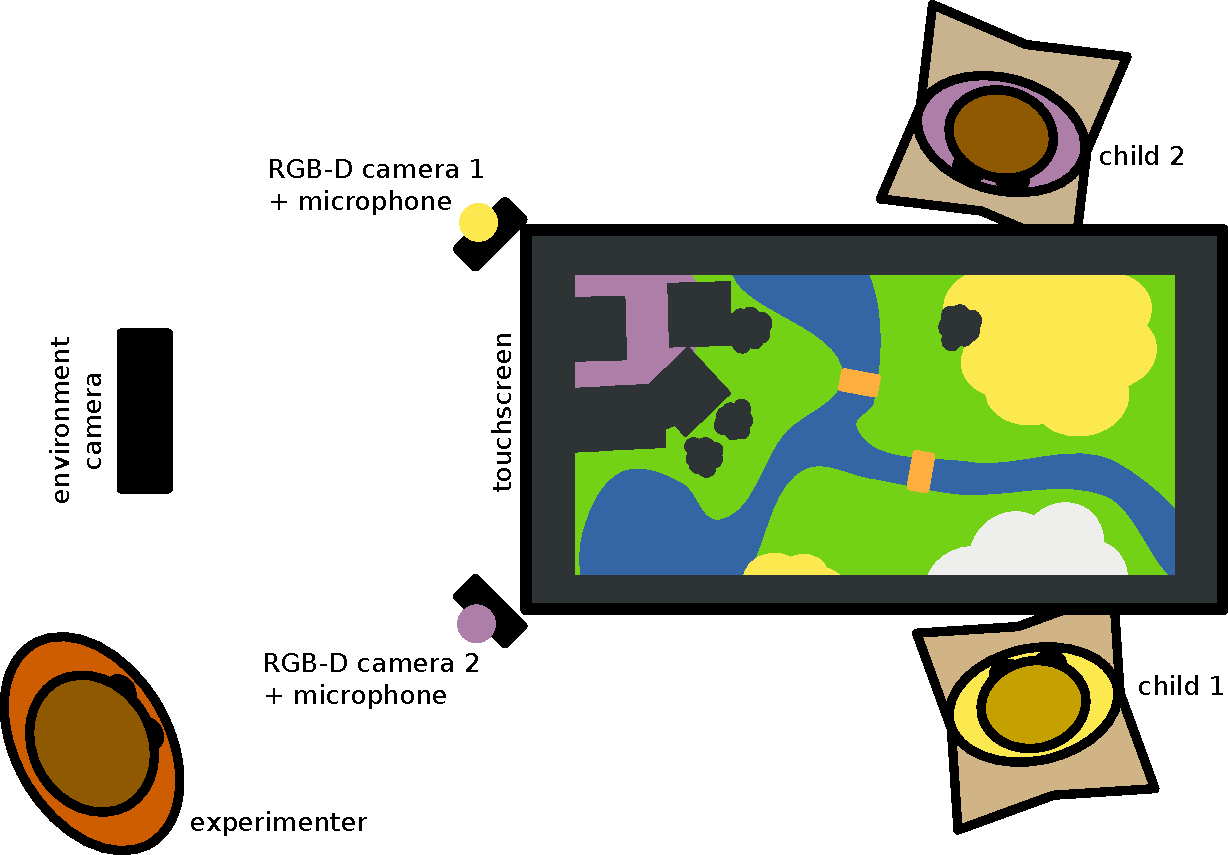
\includegraphics[width=0.8\linewidth]{setup_child_child_top}
    %\hspace{1.5cm}
    %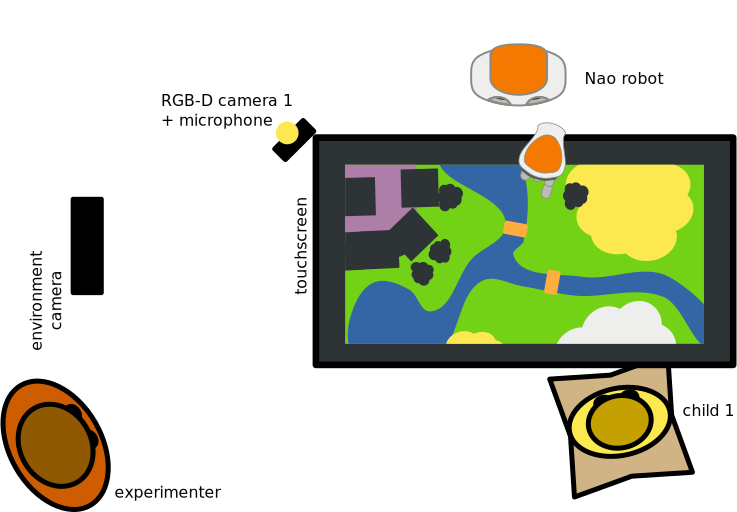
\includegraphics[width=0.4\linewidth]{setup_child_robot_top}
    %\caption{Experimental setup, child-child condition (left) and child-robot condition (right).}
    \caption{Experimental setup. Children are facing each other and sit on
    cushions. Each child wears a bright sport bib, either purple or yellow, to
    facilitate later identification.}
    \label{fig|setup}
\end{figure}

The experimenter stays in the room, visible to the child. When
requested by the nursery or school, another childminder (nursery/school
staff) can be present in the room. She/he is however asked not to step
in during the experiment.


2 age groups, balanced across conditions: 4 y.o. (nursery) and 6 to 7
y.o. (Y1/Y2)

Normally developing children, from local primary schools and nurseries.

\paragraph{Acquisition Procedure}

The following acquisition procedure has been followed with all participants.

\newcommand{\tabitem}{~~\llap{\textbullet}~~}
    \begin{tabular}{@{}p{0.2\linewidth}p{0.8\linewidth}@{}}
\toprule
\bf Welcome                       & \tabitem explain the purpose of the study: showing robots how children play  \\
\emph{(about 5 min)}              & \tabitem briefly present a Nao robot -- the robot stands up, gives a short
                                    message (\emph{"Hello, I'm Nao. Today, I'll be watching you while you
                                    play and soon I'll be able to play with you. Is that alright?"}), and
                                    sit down. The robot is then put aside and does not intervene anymore
                                    for the remaining of the experiment; \\
                                    %Condition B: "Hello, I'm Nao. Today I'll be playing with you. Exciting!")\\ 
                                  & \tabitem place children on cushions  \\ 
                                  & \tabitem give them the yellow/purple sport
                                  bibs and make sure their hair is tied \\ 
                                  & \tabitem complete demographics on the tablet \\
                                  & \tabitem remind the children that they can withdraw at anytime \\ \midrule
\bf Visual focus task             &  \\ 
\emph{(30 sec)}                   &  \\ \midrule
\bf Tutorial                      & explain how to interact with the game, ensure the children are confident with the manipulation/drawing \\ 
\emph{(1-2 min)}                  &  \\ \midrule
\bf Item placement game           &  \\
\emph{(5 to 10 min)}              &  \\ \midrule
\bf Freeplay task                 & \tabitem start the recording \\
\emph{(up to 40 min)}             & \tabitem initial prompt: \emph{"Just to remind you, you can use the animals or draw. Whatever you
                                  like. If you run out of ideas, there's also an ideas box. For example, the first one is a
                                  zoo. You could draw a zoo or tell a story. When you get bored or don't want to play
                                  anymore, just let me know."} \\
                                  & \tabitem let children play \\
                                  & \tabitem once they wish to stop, stop recording \\ \midrule
\bf Debriefing                    &  \tabitem answer possible questions from the children \\
\emph{(about 2 min)}              & \tabitem give stickers as a thank you \\ \bottomrule
\end{tabular}


\subsection{Data post-processing}

While
the raw RGB and depth streams are neither rectified nor registered together (due
to performance considerations during the recording), it can be easily achieved
as a post-process step, using standard ROS tools (the ROS {\tt rgbd\_pipeline}).
Pre-configured scripts are available alongside the dataset\footnote{Available
online from
\url{https://github.com/severin-lemaignan/freeplay-sandbox-analysis}.} to
republish registered streams and the corresponding 3D point-clouds (as seen in
Fig.~\ref{fig|rviz}, left).

Using the {\tt gazr} face tracking library\footnote{Available online from
\url{https://github.com/severin-lemaignan/gazr}. {\tt gazr} relies on the {\tt
dlib} face tracker for facial features
extraction.}~\cite{lemaignan2016realtime}, children faces and facial features can
are extracted and reprojected onto the 3D point-clouds (Fig.~\ref{fig|rviz},
right). Faces have been successfully detected in 56\% of the recorded frames
in the dataset. Undetected faces are due to occlusions (the child put her arm in
front of the camera), large head rotations or quick child motion.

\subsection{Annotations of Social Behaviours}

The last part of the dataset consist in annotations of the
children's social behaviours. Some of these behaviours are automatically
computed and coded (mutual gaze, for instance), some are human-coded.

The annotations are integrated in the dataset as a timestamped datastream.

\paragraph{Human-coded social behaviours}

We use the \emph{Social Communication Coding System} proposed by
Olswang~\etal\cite{olswang2006reliability}. It consists in 6 constructs
characterising social communication (table~\ref{table|sccs}).

% Please add the following required packages to your document preamble:
% \usepackage{booktabs}
\begin{table}[]
\centering
\caption{Constructs of the Social Communication Coding System (SCCS), taken from~\cite{olswang2006reliability}}
\label{table|sccs}
\renewcommand{\arraystretch}{1.8}
\begin{tabular}{@{}lp{0.8\linewidth}@{}}
\toprule
\bf Construct          & \bf Description                                                                                                                                                                                                                                                                                                                                           \\ \midrule
Hostile/coercive   & anti-social behavior ; examples include grabbing, hitting, taunting, provoking, yelling.                                                       \\
Prosocial/engaged  & engaged in a positive social interaction ; examples include on-task work or conversations, helping, sharing, and compromising.                 \\
Assertive          & child stating a position or opinion ; examples include asserting beliefs (verbally or nonverbally), directing the partner.                     \\
Passive/disengaged & lack of involvement in the, activity, physical disengagement ; examples include staring into space, putting head down, speaking quite softly, and walking away from an activity.\\
Adult seeking      & effort to seek assistance or attention from an adult ; examples include requesting help.                                                       \\
Irrelevant         & child being actively engaged in an off-task behavior ; examples include starting a different activity, fiddling with objects as a main focus of attention, goofy or silly behaviors. \\ \bottomrule
\end{tabular}
\end{table}



\begin{figure}
    \centering
    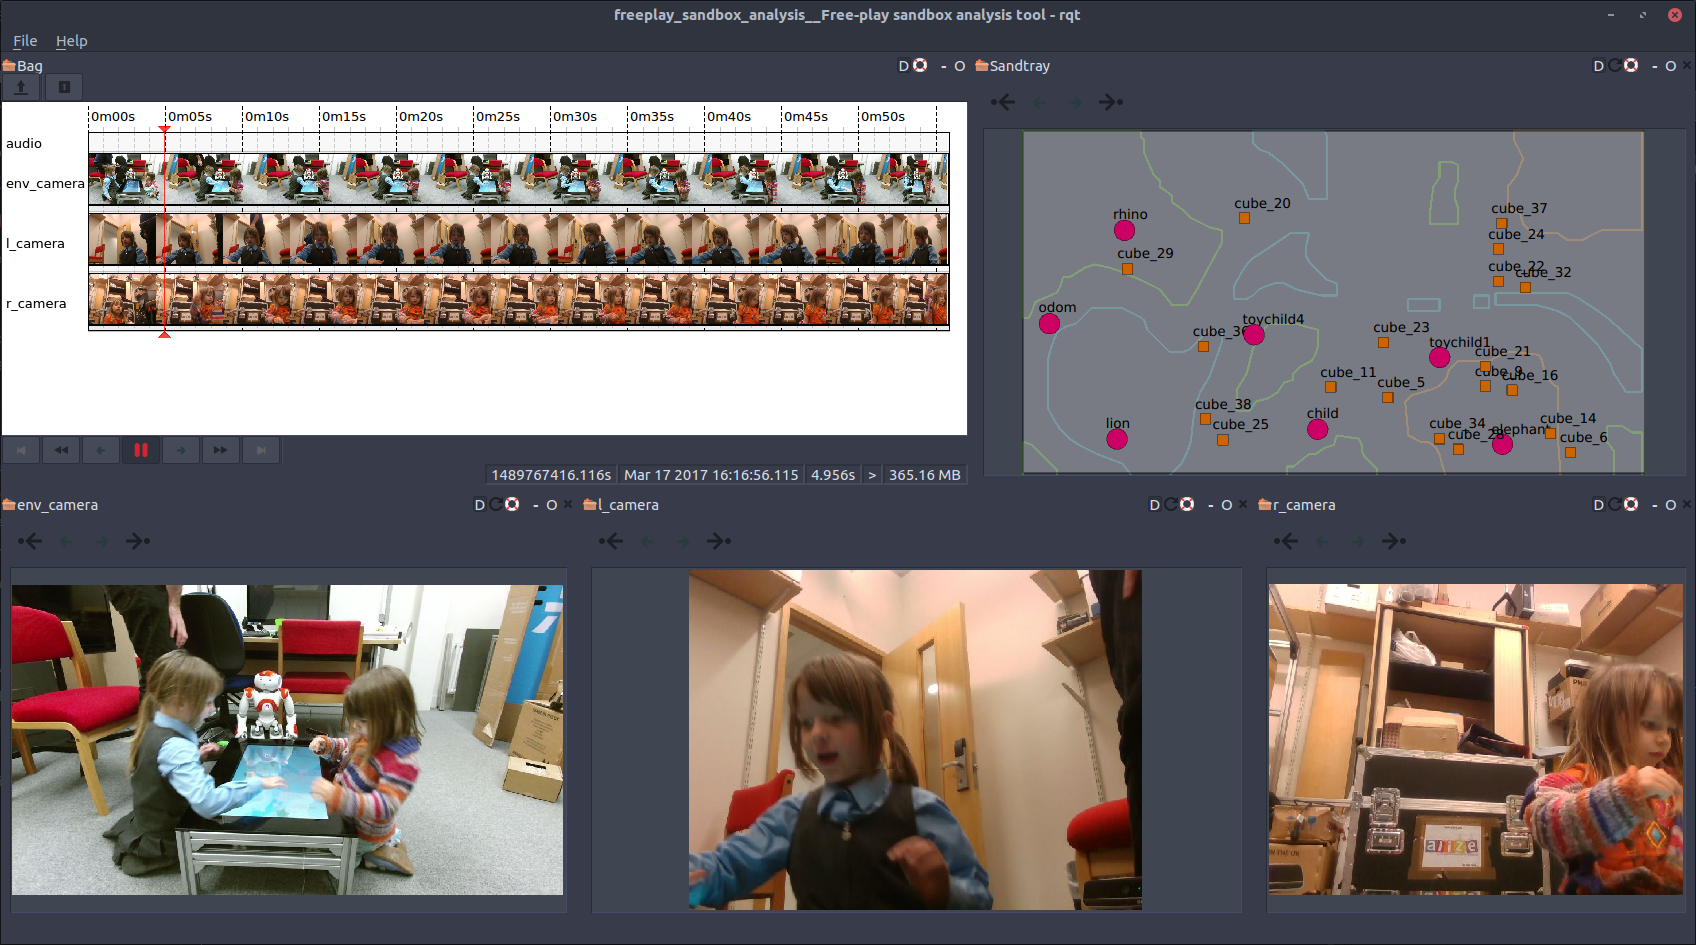
\includegraphics[width=0.8\linewidth]{analysis}
    \caption{Screenshot of the interaction analysis tool: key record information
    are played back in a synchronised (faces and audio of the two children,
    interaction occuring on the interactive table, etc.) while the human coder
    annotate the record timeline with social situations of interest.}
    \label{fig|analysis}
\end{figure}

Several metrics and coding scheme

analysis of behavioural alignment between partners (via
metrics like the recently proposed \emph{Individual Motor
Signature}~\cite{slowinski2016dynamic})

Słowinski’s Individual Motor Signature
(for behavioural alignment), Anderson's~\cite{anderson2004social} coding of children’s free-play
interactions,


\subsection{Ethical considerations and dataset availability}
\label{availability}

All data has been collected by researchers at the Plymouth University, under a
protocol approved by the university ethics committee. The parents of the
participants explicitly consented to sharing of their child's video and audio
with the research community. The data is labelled with a unique participant code
only and does not contain any identifying information, except the participant's
images. The child's age and gender are also available.

The dataset is freely available to any interested researcher\footnote{Note to
the reviewers: the link to the dataset's dedicated website will be added to the
final version of the article.}. Due to ethical and data protection regulations,
the dataset is however made available in two forms: a public, Creative-Commons
licensed, version that do not include any video material of the children (no
video streams, audio included); and a complete version that includes all video
streams. This second version is freely available as well, but interested
researchers must first fill a data protection form.


%\section{Applications}
%
%\subsection{Specific research questions}
%
%\begin{figure}
%\centering
%
%\resizebox{0.8\linewidth}{!}{%
%\begin{tikzpicture}[
%                font=\sffamily,
%                >=latex,
%                every edge/.style={draw, very thick},
%                node/.style={draw, rounded corners, align=center, inner sep=5pt, fill=black!20},
%                label/.style={midway, align=center, font=\scriptsize\sffamily, fill=white}]
%
%    %%% NODES
%    \node [node] (mentalrepresentations) {Mental Representations};
%    \node [above left=of mentalrepresentations] (gameactions) {\it game actions};
%    \node [node, above=of gameactions] (gamedynamics) {Game dynamics};
%    \node [above right=of mentalrepresentations] (socialactions) {\it social actions};
%    \node [node, above=of socialactions ] (socialdynamics) {Social Dynamics};
%
%    %%% CONNECTIONS
%    \path (gamedynamics) edge [<->, dashed] node[label, above] {?}(socialdynamics);
%    \path (gamedynamics) edge [<-, bend right] node[label] {mediate}(gameactions);
%    \path (socialactions) edge [->, bend left] node[label] {reflect}(mentalrepresentations);
%    \path (socialactions) edge [->, dashed] node[label,above] {?}(gamedynamics);
%    \path (gameactions) edge [->, dashed] node[label,above] {?}(socialdynamics);
%    \path (gameactions) edge [->, bend right] node[label] {reflect}(mentalrepresentations);
%    \path (socialdynamics) edge [<-, bend left] node[label] {shape}(socialactions);
%
%\end{tikzpicture}
%}
%\label{fig|researchquestions}
%\caption{Game dynamics, social dynamics and mental representations are linked
%    with each other through social actions (implicit and explicit communication)
%    and actions on the environment (mainly game actions)}
%\end{figure}
%
%The mechanisms underlying the social interactions happening during free play
%raise important questions for social robotics.
%
%
%\subsubsection{Game Dynamics}
%
%\begin{itemize}
%    \item do we observe a sequence of sub-games?
%    \item how are these sub-games initiated?
%    \item how does A keep track of what B is playing at?
%    \item how do we segment the action flow into meaningful play situations?
%\end{itemize}
%
%\subsubsection{Social Dynamics}
%
%\begin{itemize}
%    \item does a ``social protocol'' establish?
%    \item if so, what are these social rules?
%    \item implicit vs explicit rule setting?
%    \item what interaction modalities (or combination thereof) are relied upon
%        to establish and maintain this ``social protocol''?
%\end{itemize}
%
%\subsubsection{Mental representations}
%
%\begin{itemize}
%    \item Does A know what B is thinking of at time t?
%    \item Do the participants perform explicit grounding of their respective mental models
%        (ie, ask the other one what she is doing/thinking/planning to do?)
%    \item How does the implicit grounding take place? attention tracking?
%    \item Do we need at all to know what the other intends to do to actually
%        collaborate? surface alignment vs deep grounding
%    \item Procedural (how do you do it?) vs Semantic
%        grounding (what are you doing? playing at?)
%\end{itemize}

\subsection{Child-robot baseline}

During the acquisition campaign for the PInSoRo dataset, we have also recorded a
\emph{child-robot} interaction baseline. We were using the exact same protocol
as described above, only with one child replaced by a Nao robot.

The robot was fully autonomous, and programmed to exhibit a non-social behaviour
(its action policy was simply to repeatedly move interactive items to
pre-defined zones, entirely ignoring its child partner).

As such, this behaviour (and the resulting reaction of the children to a
robot acting in a non-social way) represent an experimental baseline against which
future work can be compared.


%\subsection{Analysis of the free play sandbox}
%
%Our free play sandbox elicits a loosely structured play situation. The
%situation is indeed essentially aimless (free play). The goals and play episodes
%that we observe during the interactions are not pre-defined, and essentially
%unknown until they are decided by the players. In this sense, the free play
%sandbox permits and elicits what is fundamentally \emph{unstructured play}.
%
%However, a second look reveals some important structuring elements.
%
%First, the physical bounds of the sandbox (an interactive table) limit the
%play zone to a well defined and relatively small area. As a consequence,
%children are mostly static (they are sitting in front of the table) and their
%primary form of interaction is 2D pick and place of items by drag and dropping
%them on the screen.
%
%Second, the game items themselves structure the game scenarios. Items are either
%iconic characters (animals or children) or plain blocks
%(Figure~\ref{fig|sandbox}). The former have strong semantics associated to them
%(like 'crocodiles like water and eat children'), while the later have little
%semantics associated. The game background, with its recognizable zones, also
%elicit a particular type of games (like building a zoo or pretending we explore
%the savannah).
%
%Two more elements (the role and place of the experimenter, and the initial
%prompt given to the participant) have an important impact on the shape of the
%play situation. We discuss separately these two points in the description of the
%experimental procedure.
%
%Overall, the free play sandbox supports a \emph{loosely structured} form of play: the
%actual play situations are not known and might change several times during the
%interaction; the game actions, even though all based on a single modality (picking and
%placing game items), are unlimited; the social interactions between participants
%are multi-modal (speech, body postures, gestures, facial expressions, etc.) and
%unconstrainted. However, the broad domain of the play situations and the range of
%possible social interactions is bound by the physical bounds of the play zone
%and the theme of the game items.
%
%\subsection{Forms of play elicited by the sandbox}
%
%\begin{itemize}
%    \item dramatic play
%    \item storytelling
%    \item creative play
%    \item pretend play
%\end{itemize}
%

\section{Conclusion}
%
%
%By analyzing them from the
%perspective of artifical socio-cognition and human-robot interaction, we
%evidence key social patterns and show that robots can recognise them,
%interpret them, and (where applicable) generate them in a task-agnostic
%fashion. By subsequently reusing these social patterns in similar
%child-robot free play situations, we show a significant increase of the
%interaction duration.

We introduce a novel dataset for the study of social cognition. The dataset
consists in dyadic free-play episodes, with children aged 4 to 8.

The dataset is build with machine learning applications in mind, and
particularly, applications to socio-cognitive robotics.


Finally, the social setting (two players facing each other) implicitely invites
social interaction: onlooker play, for instance, is unlikely to be observed as
the children are physically engaged with the game and the other participant
(they are sitting in front of game, close to each other). The three higher forms
of social play listed by Parten (parallel play, associative play and cooperative
play) are however possible with this setup.



\bibliography{biblio}

\end{document}
